%version 1.00,	date 12/05/2016	auteur(s) Pierre Porche
\speaker{\Mathieu}

\begin{frame}
\frametitle{M\underline{V}C : Les vues}
\begin{figure}[!h]
	\begin{center}
	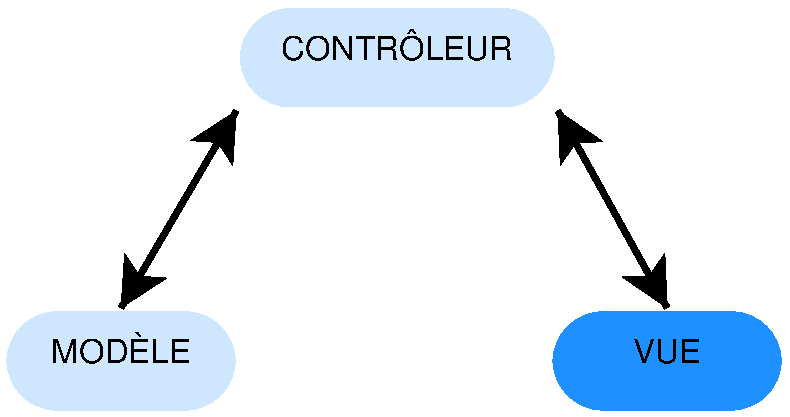
\includegraphics[scale=0.5]{images/mvcVue}
	\caption{Architecture M\underline{V}C}
	\end{center}
\end{figure}
\end{frame}

\begin{frame}
\frametitle{M\underline{V}C : Les vues}
\begin{block}{Vocabulaire}
\textbf{Template} : définit l'habillage d'une page, la position de ses éléments
\end{block}
\begin{figure}[!h]
	\begin{center}
	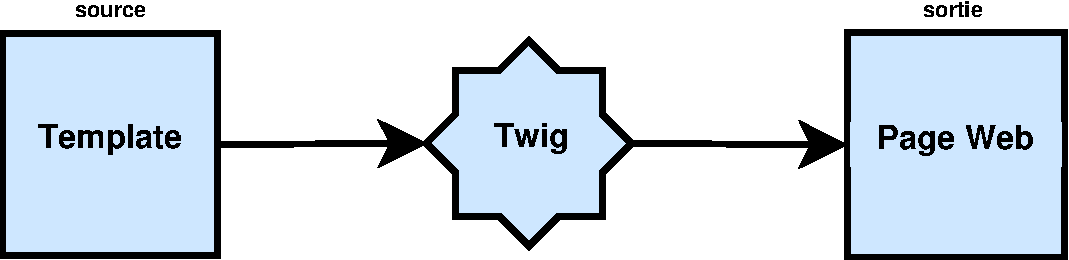
\includegraphics[scale=0.5]{images/twig}
	\caption{Fonctionnement du moteur de template Twig}
	\end{center}
\end{figure}
\end{frame}

\begin{frame}
\frametitle{M\underline{V}C : Les vues}
\begin{block}{Architecture des templates}
	\begin{itemize}
		\item Niveau 1 : architecture générale pour l'ensemble des pages
		\item Niveau 2 : architecture spécifique pour chaque groupe de pages similaires
		\item Niveau 3 : templates finaux pour chaque page Web de l'application
	\end{itemize}
\end{block}
\begin{figure}[!h]
	\begin{center}
	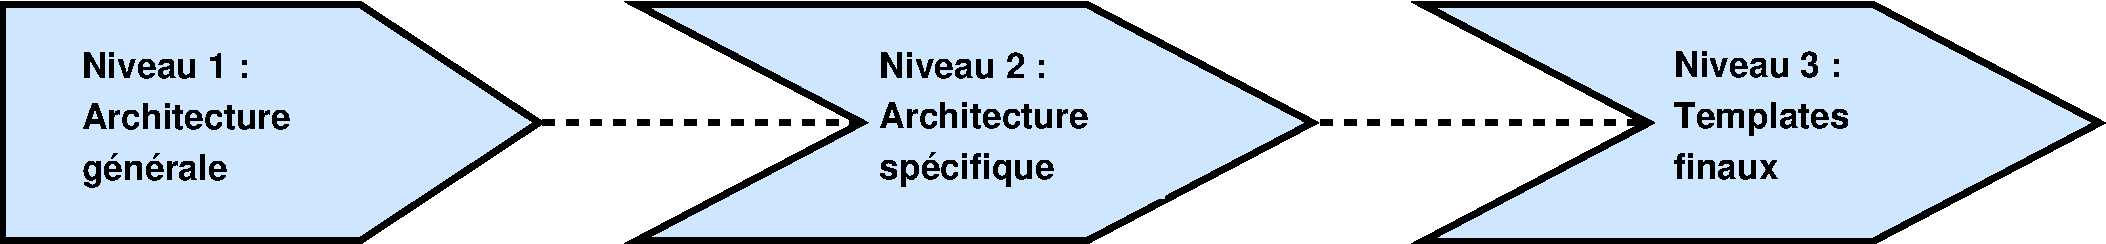
\includegraphics[scale=0.3]{images/archiTemplates}
	\caption{Imbrication des templates}
	\end{center}
\end{figure}
\end{frame}

\begin{frame}
\frametitle{M\underline{V}C : Les vues}
\begin{block}{Utilisation d'une collection d'outils CSS : Bootstrap}
	\begin{itemize}
		\item Gain de temps
		\item Prise en charge native par Symfony
		\item Application accessible depuis tout type d'appareil (ordinateur, tablette, smartphone)
	\end{itemize}
\end{block}
\end{frame}

\begin{frame}[plain]
\begin{figure}[!h]
	\begin{center}
	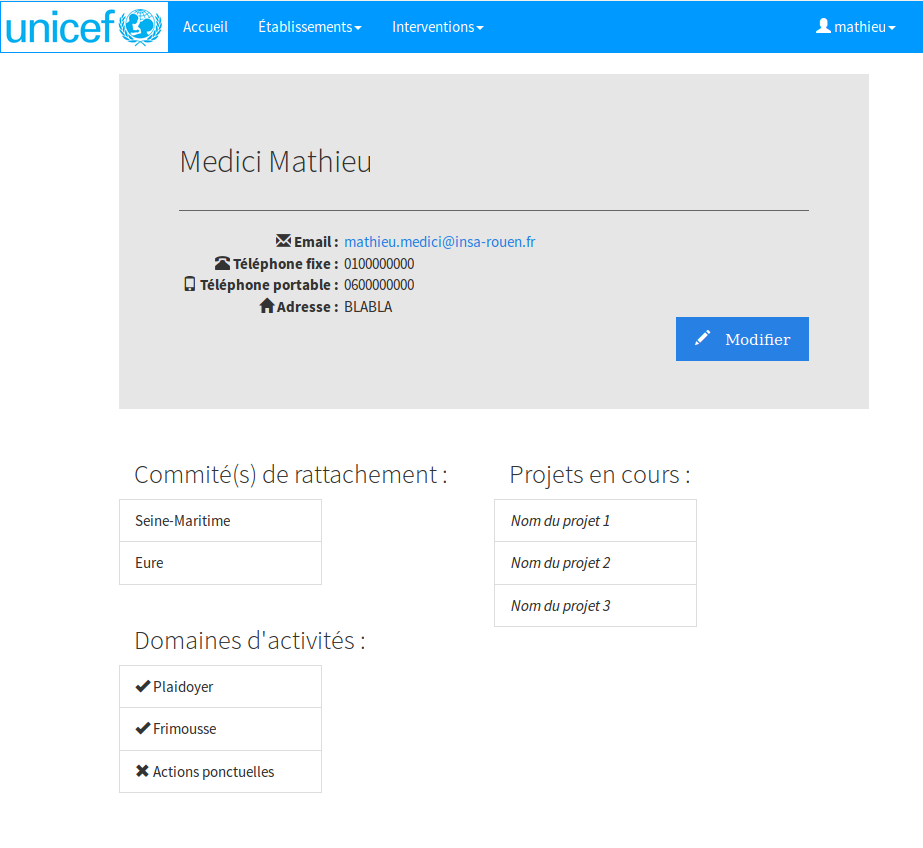
\includegraphics[scale=0.25]{images/profil.png}
	\caption{Page web du profil d'un utilisateur}
	\end{center}
\end{figure}
\end{frame}

\begin{frame}[plain]
\begin{figure}[!h]
	\begin{center}
	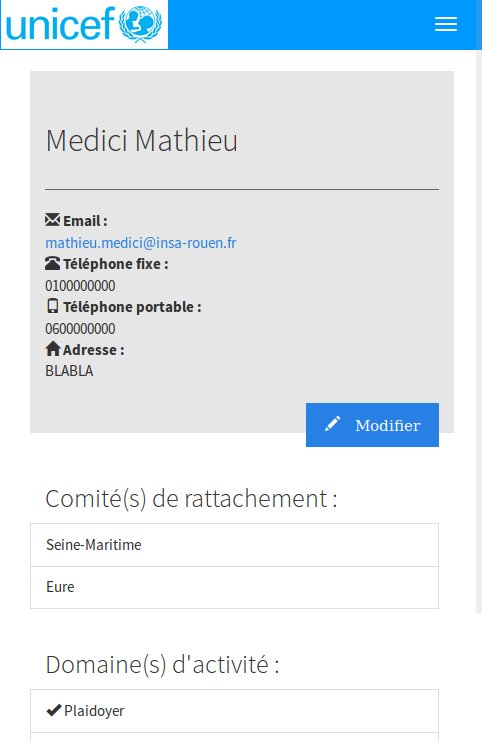
\includegraphics[scale=0.25]{images/profilSmartphone.png}
	\caption{Page web sur smartphone du profil d'un utilisateur}
	\end{center}
\end{figure}
\end{frame}